\chapter{همبندی قوی}

\index{گراف قویاً همبند}

در گراف جهت‌دار،
یال‌ها فقط در یک جهت پیمایش می‌شوند؛
بنابراین حتی اگر گراف همبند باشد،
وجود مسیر بین هر دو گره تضمین نمی‌شود.
به همین دلیل، تعریف مفهومی قوی‌تر از همبندی نیاز است.

گراف \key{قویاً همبند} است
اگر بین هر گره و تمام گره‌های دیگر
مسیر وجود داشته باشد.
برای نمونه، در تصویر زیر،
گراف سمت چپ قویاً همبند است
ولی گراف سمت راست نیست.

\begin{center}
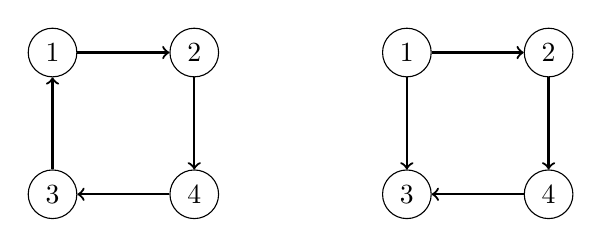
\begin{tikzpicture}[scale=0.9]
\node[draw, circle] (1) at (1,1) {$1$};
\node[draw, circle] (2) at (3,1) {$2$};
\node[draw, circle] (3) at (1,-1) {$3$};
\node[draw, circle] (4) at (3,-1) {$4$};

\path[draw,thick,->] (1) -- (2);
\path[draw,thick,->] (2) -- (4);
\path[draw,thick,->] (4) -- (3);
\path[draw,thick,->] (3) -- (1);

\node[draw, circle] (1b) at (6,1) {$1$};
\node[draw, circle] (2b) at (8,1) {$2$};
\node[draw, circle] (3b) at (6,-1) {$3$};
\node[draw, circle] (4b) at (8,-1) {$4$};

\path[draw,thick,->] (1b) -- (2b);
\path[draw,thick,->] (2b) -- (4b);
\path[draw,thick,->] (4b) -- (3b);
\path[draw,thick,->] (1b) -- (3b);
\end{tikzpicture}
\end{center}

گراف سمت راست قویاً همبند نیست
چون مثلاً مسیری
از گره 2 به گره 1 وجود ندارد.

\index{مؤلفه قویاً همبند}
\index{گراف مؤلفه‌ها}

\key{مؤلفه‌های قویاً همبند}
یک گراف، آن را به بزرگ‌ترین بخش‌های قویاً همبند
افراز می‌کنند.
این مؤلفه‌ها یک \key{گراف مؤلفه‌ها}ی بدون دور تشکیل می‌دهند
که ساختار عمیق گراف اصلی را نشان می‌دهد.

برای نمونه، در گراف
\begin{center}
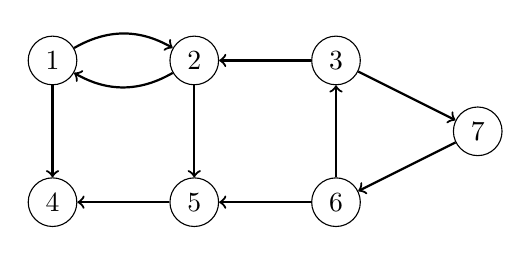
\begin{tikzpicture}[scale=0.9,label distance=-2mm]
\node[draw, circle] (1) at (-1,1) {$7$};
\node[draw, circle] (2) at (-3,2) {$3$};
\node[draw, circle] (4) at (-5,2) {$2$};
\node[draw, circle] (6) at (-7,2) {$1$};
\node[draw, circle] (3) at (-3,0) {$6$};
\node[draw, circle] (5) at (-5,0) {$5$};
\node[draw, circle] (7) at (-7,0) {$4$};

\path[draw,thick,->] (2) -- (1);
\path[draw,thick,->] (1) -- (3);
\path[draw,thick,->] (3) -- (2);
\path[draw,thick,->] (2) -- (4);
\path[draw,thick,->] (3) -- (5);
\path[draw,thick,->] (4) edge [bend left] (6);
\path[draw,thick,->] (6) edge [bend left] (4);
\path[draw,thick,->] (4) -- (5);
\path[draw,thick,->] (5) -- (7);
\path[draw,thick,->] (6) -- (7);
\end{tikzpicture}
\end{center}
مؤلفه‌های قویاً همبند این‌گونه هستند:
\begin{center}
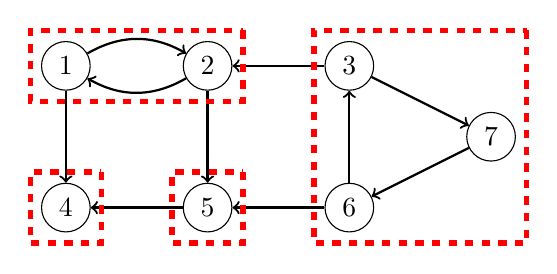
\begin{tikzpicture}[scale=0.9]
\node[draw, circle] (1) at (-1,1) {$7$};
\node[draw, circle] (2) at (-3,2) {$3$};
\node[draw, circle] (4) at (-5,2) {$2$};
\node[draw, circle] (6) at (-7,2) {$1$};
\node[draw, circle] (3) at (-3,0) {$6$};
\node[draw, circle] (5) at (-5,0) {$5$};
\node[draw, circle] (7) at (-7,0) {$4$};

\path[draw,thick,->] (2) -- (1);
\path[draw,thick,->] (1) -- (3);
\path[draw,thick,->] (3) -- (2);
\path[draw,thick,->] (2) -- (4);
\path[draw,thick,->] (3) -- (5);
\path[draw,thick,->] (4) edge [bend left] (6);
\path[draw,thick,->] (6) edge [bend left] (4);
\path[draw,thick,->] (4) -- (5);
\path[draw,thick,->] (5) -- (7);
\path[draw,thick,->] (6) -- (7);

\draw [red,thick,dashed,line width=2pt] (-0.5,2.5) rectangle (-3.5,-0.5);
\draw [red,thick,dashed,line width=2pt] (-4.5,2.5) rectangle (-7.5,1.5);
\draw [red,thick,dashed,line width=2pt] (-4.5,0.5) rectangle (-5.5,-0.5);
\draw [red,thick,dashed,line width=2pt] (-6.5,0.5) rectangle (-7.5,-0.5);
\end{tikzpicture}
\end{center}
گراف مؤلفه‌ای متناظر به صورت زیر است:
\begin{center}
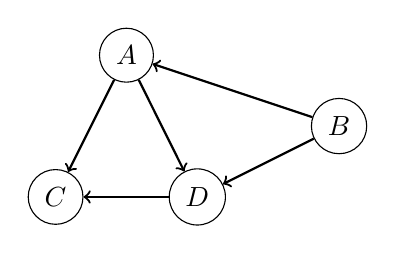
\begin{tikzpicture}[scale=0.9]
\node[draw, circle] (1) at (-3,1) {$B$};
\node[draw, circle] (2) at (-6,2) {$A$};
\node[draw, circle] (3) at (-5,0) {$D$};
\node[draw, circle] (4) at (-7,0) {$C$};

\path[draw,thick,->] (1) -- (2);
\path[draw,thick,->] (1) -- (3);
\path[draw,thick,->] (2) -- (3);
\path[draw,thick,->] (2) -- (4);
\path[draw,thick,->] (3) -- (4);
\end{tikzpicture}
\end{center}
مؤلفه‌ها عبارتند از $A=\{1,2\}$،
$B=\{3,6,7\}$، $C=\{4\}$ و $D=\{5\}$.

یک گراف مؤلفه‌ای، گرافی جهت‌دار و بدون دور است،
بنابراین پردازش آن نسبت به گراف اصلی آسان‌تر است.
از آنجا که گراف فاقد دور است،
همواره می‌توان یک مرتب‌سازی توپولوژیکی ایجاد کرد و
روش‌های برنامه‌نویسی پویا مانند روش‌های
ارائه‌شده در فصل ۱۶ را به کار برد.

\section{الگوریتم کوساراجو}

\index{الگوریتم کوساراجو}

\key{الگوریتم کوساراجو}\footnote{طبق \cite{aho83}،
اس. آر. کوساراجو این الگوریتم را در سال ۱۹۷۸ ابداع کرد
ولی آن را منتشر نکرد. در سال ۱۹۸۱، همین الگوریتم مجدداً
توسط ام. شریر کشف و منتشر شد \cite{sha81}.} روشی کارآمد
برای یافتن مؤلفه‌های قویاً همبند
یک گراف جهت‌دار است.
الگوریتم دو جستجوی اول‌سطح‌عمق انجام می‌دهد:
جستجوی اول فهرستی از گره‌ها را با توجه به ساختار گراف می‌سازد،
و جستجوی دوم مؤلفه‌های قویاً همبند را تشکیل می‌دهد.

\subsubsection{جستجوی ۱}

مرحله اول الگوریتم کوساراجو،
فهرستی از گره‌ها را به ترتیبی که جستجوی اول‌سطح‌عمق آن‌ها را پردازش می‌کند، می‌سازد.
الگوریتم روی گره‌ها پیمایش می‌کند،
و در هر گره پردازش‌نشده یک جستجوی اول‌سطح‌عمق را آغاز می‌کند.
هر گره پس از پردازش،
به فهرست اضافه می‌شود.

در گراف نمونه، گره‌ها
به ترتیب زیر پردازش می‌شوند:
\begin{center}
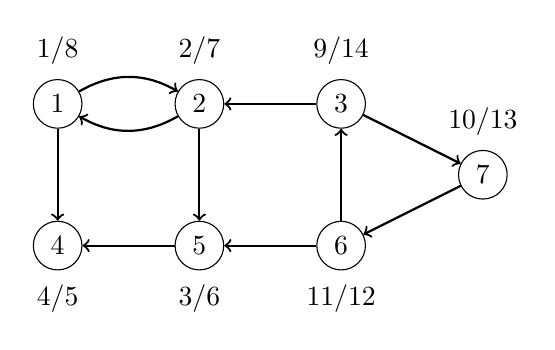
\begin{tikzpicture}[scale=0.9,label distance=-2mm]
\node[draw, circle] (1) at (-1,1) {$7$};
\node[draw, circle] (2) at (-3,2) {$3$};
\node[draw, circle] (4) at (-5,2) {$2$};
\node[draw, circle] (6) at (-7,2) {$1$};
\node[draw, circle] (3) at (-3,0) {$6$};
\node[draw, circle] (5) at (-5,0) {$5$};
\node[draw, circle] (7) at (-7,0) {$4$};

\node at (-7,2.75) {$1/8$};
\node at (-5,2.75) {$2/7$};
\node at (-3,2.75) {$9/14$};
\node at (-7,-0.75) {$4/5$};
\node at (-5,-0.75) {$3/6$};
\node at (-3,-0.75) {$11/12$};
\node at (-1,1.75) {$10/13$};

\path[draw,thick,->] (2) -- (1);
\path[draw,thick,->] (1) -- (3);
\path[draw,thick,->] (3) -- (2);
\path[draw,thick,->] (2) -- (4);
\path[draw,thick,->] (3) -- (5);
\path[draw,thick,->] (4) edge [bend left] (6);
\path[draw,thick,->] (6) edge [bend left] (4);
\path[draw,thick,->] (4) -- (5);
\path[draw,thick,->] (5) -- (7);
\path[draw,thick,->] (6) -- (7);
\end{tikzpicture}
\end{center}

نمادگذاری $x/y$ یعنی
پردازش رأس در زمان $x$ شروع
و در زمان $y$ پایان یافت.
بنابراین لیست متناظر بدین صورت است:

\begin{tabular}{ll}
\\
رأس & زمان پردازش \\
\hline
4 & 5 \\
5 & 6 \\
2 & 7 \\
1 & 8 \\
6 & 12 \\
7 & 13 \\
3 & 14 \\
\\
\end{tabular}
% 
% In the second phase of the algorithm,
% the nodes will be processed
% in reverse order: $[3,7,6,1,2,5,4]$.

\subsubsection{جستجوی ۲}

مرحله دوم الگوریتم،
مؤلفه‌های قویاً همبند گراف را تشکیل می‌دهد.
ابتدا الگوریتم تمام یال‌های گراف را معکوس می‌کند.
این کار تضمین می‌کند که طی جستجوی دوم،
همواره مؤلفه‌های قویاً همبندی بدون رأس‌های اضافه پیدا کنیم.

پس از معکوس کردن یال‌ها،
گراف نمونه بدین صورت درمی‌آید:
\begin{center}
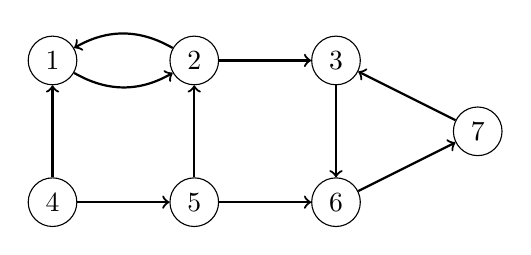
\begin{tikzpicture}[scale=0.9,label distance=-2mm]
\node[draw, circle] (1) at (-1,1) {$7$};
\node[draw, circle] (2) at (-3,2) {$3$};
\node[draw, circle] (4) at (-5,2) {$2$};
\node[draw, circle] (6) at (-7,2) {$1$};
\node[draw, circle] (3) at (-3,0) {$6$};
\node[draw, circle] (5) at (-5,0) {$5$};
\node[draw, circle] (7) at (-7,0) {$4$};

\path[draw,thick,<-] (2) -- (1);
\path[draw,thick,<-] (1) -- (3);
\path[draw,thick,<-] (3) -- (2);
\path[draw,thick,<-] (2) -- (4);
\path[draw,thick,<-] (3) -- (5);
\path[draw,thick,<-] (4) edge [bend left] (6);
\path[draw,thick,<-] (6) edge [bend left] (4);
\path[draw,thick,<-] (4) -- (5);
\path[draw,thick,<-] (5) -- (7);
\path[draw,thick,<-] (6) -- (7);
\end{tikzpicture}
\end{center}

سپس الگوریتم لیست رأس‌های حاصل از جستجوی اول را
به ترتیب \emph{معکوس} پیمایش می‌کند.
اگر رأسی متعلق به مؤلفه‌ای نباشد،
الگوریتم مؤلفه جدیدی ایجاد می‌کند
و یک جستجوی اول‌سطح‌عمق آغاز می‌کند
که تمام رأس‌های جدید یافته‌شده طی جستجو را
به مؤلفه جدید اضافه می‌کند.

در گراف نمونه، مؤلفه نخست
از رأس ۳ آغاز می‌شود:

\begin{center}
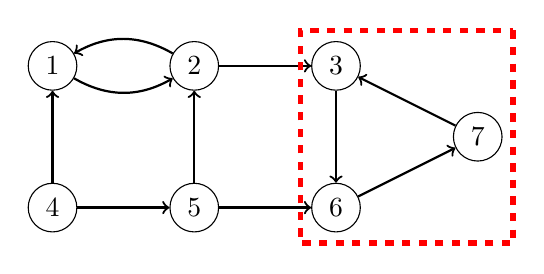
\begin{tikzpicture}[scale=0.9,label distance=-2mm]
\node[draw, circle] (1) at (-1,1) {$7$};
\node[draw, circle] (2) at (-3,2) {$3$};
\node[draw, circle] (4) at (-5,2) {$2$};
\node[draw, circle] (6) at (-7,2) {$1$};
\node[draw, circle] (3) at (-3,0) {$6$};
\node[draw, circle] (5) at (-5,0) {$5$};
\node[draw, circle] (7) at (-7,0) {$4$};

\path[draw,thick,<-] (2) -- (1);
\path[draw,thick,<-] (1) -- (3);
\path[draw,thick,<-] (3) -- (2);
\path[draw,thick,<-] (2) -- (4);
\path[draw,thick,<-] (3) -- (5);
\path[draw,thick,<-] (4) edge [bend left] (6);
\path[draw,thick,<-] (6) edge [bend left] (4);
\path[draw,thick,<-] (4) -- (5);
\path[draw,thick,<-] (5) -- (7);
\path[draw,thick,<-] (6) -- (7);

\draw [red,thick,dashed,line width=2pt] (-0.5,2.5) rectangle (-3.5,-0.5);
\end{tikzpicture}
\end{center}

توجه کنید چون تمام یال‌ها معکوس شده‌اند،
مؤلفه به بخش‌های دیگر گراف نشت نمی‌کند.

\begin{samepage}
راس‌های بعدی در لیست راس‌های 7 و 6 هستند،
اما این راس‌ها از قبل به یک مؤلفه تعلق دارند،
بنابراین مؤلفه جدید بعدی از راس 1 آغاز می‌شود:

\begin{center}
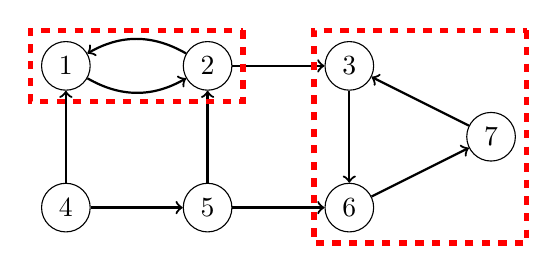
\begin{tikzpicture}[scale=0.9,label distance=-2mm]
\node[draw, circle] (1) at (-1,1) {$7$};
\node[draw, circle] (2) at (-3,2) {$3$};
\node[draw, circle] (4) at (-5,2) {$2$};
\node[draw, circle] (6) at (-7,2) {$1$};
\node[draw, circle] (3) at (-3,0) {$6$};
\node[draw, circle] (5) at (-5,0) {$5$};
\node[draw, circle] (7) at (-7,0) {$4$};

\path[draw,thick,<-] (2) -- (1);
\path[draw,thick,<-] (1) -- (3);
\path[draw,thick,<-] (3) -- (2);
\path[draw,thick,<-] (2) -- (4);
\path[draw,thick,<-] (3) -- (5);
\path[draw,thick,<-] (4) edge [bend left] (6);
\path[draw,thick,<-] (6) edge [bend left] (4);
\path[draw,thick,<-] (4) -- (5);
\path[draw,thick,<-] (5) -- (7);
\path[draw,thick,<-] (6) -- (7);

\draw [red,thick,dashed,line width=2pt] (-0.5,2.5) rectangle (-3.5,-0.5);
\draw [red,thick,dashed,line width=2pt] (-4.5,2.5) rectangle (-7.5,1.5);
%\draw [red,thick,dashed,line width=2pt] (-4.5,0.5) rectangle (-5.5,-0.5);
%\draw [red,thick,dashed,line width=2pt] (-6.5,0.5) rectangle (-7.5,-0.5);
\end{tikzpicture}
\end{center}
\end{samepage}

\begin{samepage}
در نهایت، الگوریتم راس‌های 5 و 4 را پردازش می‌کند
که مؤلفه‌های قویا همبند باقی‌مانده را تشکیل می‌دهند:

\begin{center}
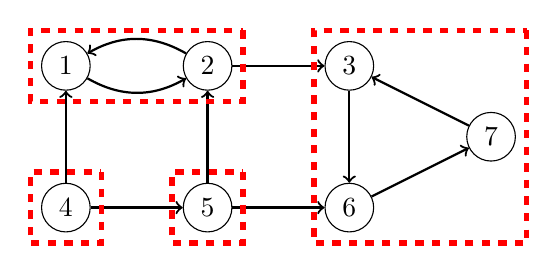
\begin{tikzpicture}[scale=0.9,label distance=-2mm]
\node[draw, circle] (1) at (-1,1) {$7$};
\node[draw, circle] (2) at (-3,2) {$3$};
\node[draw, circle] (4) at (-5,2) {$2$};
\node[draw, circle] (6) at (-7,2) {$1$};
\node[draw, circle] (3) at (-3,0) {$6$};
\node[draw, circle] (5) at (-5,0) {$5$};
\node[draw, circle] (7) at (-7,0) {$4$};

\path[draw,thick,<-] (2) -- (1);
\path[draw,thick,<-] (1) -- (3);
\path[draw,thick,<-] (3) -- (2);
\path[draw,thick,<-] (2) -- (4);
\path[draw,thick,<-] (3) -- (5);
\path[draw,thick,<-] (4) edge [bend left] (6);
\path[draw,thick,<-] (6) edge [bend left] (4);
\path[draw,thick,<-] (4) -- (5);
\path[draw,thick,<-] (5) -- (7);
\path[draw,thick,<-] (6) -- (7);

\draw [red,thick,dashed,line width=2pt] (-0.5,2.5) rectangle (-3.5,-0.5);
\draw [red,thick,dashed,line width=2pt] (-4.5,2.5) rectangle (-7.5,1.5);
\draw [red,thick,dashed,line width=2pt] (-4.5,0.5) rectangle (-5.5,-0.5);
\draw [red,thick,dashed,line width=2pt] (-6.5,0.5) rectangle (-7.5,-0.5);
\end{tikzpicture}
\end{center}
\end{samepage}

پیچیدگی زمانی الگوریتم $O(n+m)$ است،
چرا که الگوریتم
دو جستجوی اول عمق انجام می‌دهد.

\section{مسئله 2SAT}

\index{مسئله 2SAT}

همبندی قوی با \key{مسئله 2SAT}\footnote{الگوریتم ارائه‌شده در اینجا در \cite{asp79} معرفی شد. الگوریتم زمان‌خطی شناخته‌شده دیگری نیز بر پایه عقب‌گرد (backtracking) وجود دارد \cite{eve75}.} مرتبط است.
در این مسئله، فرمول منطقی زیر داده می‌شود:
\[
(a_1 \lor b_1) \land (a_2 \lor b_2) \land \cdots \land (a_m \lor b_m),
\]
که هر $a_i$ و $b_i$ متغیر منطقی ($x_1,x_2,\ldots,x_n$) یا نقیض متغیر منطقی ($\lnot x_1, \lnot x_2, \ldots, \lnot x_n$) است.
نمادهای ''$\land$'' و ''$\lor$'' نشان‌دهنده عملگرهای منطقی «و» و «یا» هستند.
هدف، مقداردهی به متغیرها برای صدق فرمول، یا اعلام عدم امکان آن است.

مثال: فرمول
\[
L_1 = (x_2 \lor \lnot x_1) \land
      (\lnot x_1 \lor \lnot x_2) \land
      (x_1 \lor x_3) \land
      (\lnot x_2 \lor \lnot x_3) \land
      (x_1 \lor x_4)
\]
با مقداردهی زیر درست است:

\[
\begin{cases}
x_1 = \textrm{false} \\
x_2 = \textrm{false} \\
x_3 = \textrm{true} \\
x_4 = \textrm{true} \\
\end{cases}
\]

اما فرمول
\[
L_2 = (x_1 \lor x_2) \land
      (x_1 \lor \lnot x_2) \land
      (\lnot x_1 \lor x_3) \land
      (\lnot x_1 \lor \lnot x_3)
\]
با هر مقداردهی نادرست است.
دلیل: انتخاب مقدار برای $x_1$ بدون تناقض ممکن نیست.
اگر $x_1$ نادرست باشد، هر دو $x_2$ و $\lnot x_2$ باید درست باشند که ناممکن است.
اگر $x_1$ درست باشد، هر دو $x_3$ و $\lnot x_3$ باید درست باشند که این نیز ناممکن است.

مسئله 2SAT با گرافی مدل می‌شود که رأس‌های آن متغیرهای $x_i$ و نقیض‌هایشان $\lnot x_i$ هستند، و یال‌ها روابط بین متغیرها را تعیین می‌کنند.
هر مؤلفه $(a_i \lor b_i)$ دو یال ایجاد می‌کند:
$\lnot a_i \to b_i$ و $\lnot b_i \to a_i$.
یعنی اگر $a_i$ برقرار نباشد، $b_i$ باید برقرار باشد، و برعکس.

گراف فرمول $L_1$:
\\
\begin{center}
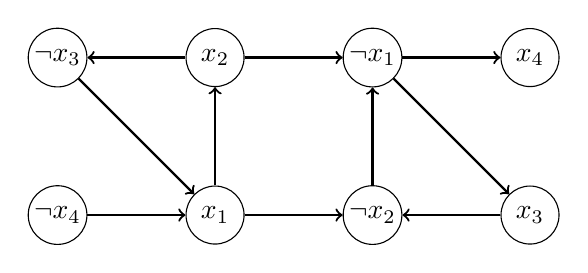
\begin{tikzpicture}[scale=1.0,minimum size=2pt]
\node[draw, circle, inner sep=1.3pt] (1) at (1,2) {$\lnot x_3$};
\node[draw, circle] (2) at (3,2) {$x_2$};
\node[draw, circle, inner sep=1.3pt] (3) at (1,0) {$\lnot x_4$};
\node[draw, circle] (4) at (3,0) {$x_1$};
\node[draw, circle, inner sep=1.3pt] (5) at (5,2) {$\lnot x_1$};
\node[draw, circle] (6) at (7,2) {$x_4$};
\node[draw, circle, inner sep=1.3pt] (7) at (5,0) {$\lnot x_2$};
\node[draw, circle] (8) at (7,0) {$x_3$};
 
\path[draw,thick,->] (1) -- (4);
\path[draw,thick,->] (4) -- (2);
\path[draw,thick,->] (2) -- (1);
\path[draw,thick,->] (3) -- (4);
\path[draw,thick,->] (2) -- (5);
\path[draw,thick,->] (4) -- (7);
\path[draw,thick,->] (5) -- (6);
\path[draw,thick,->] (5) -- (8);
\path[draw,thick,->] (8) -- (7);
\path[draw,thick,->] (7) -- (5);
\end{tikzpicture}
\end{center}
گراف فرمول $L_2$:
\\
\begin{center}
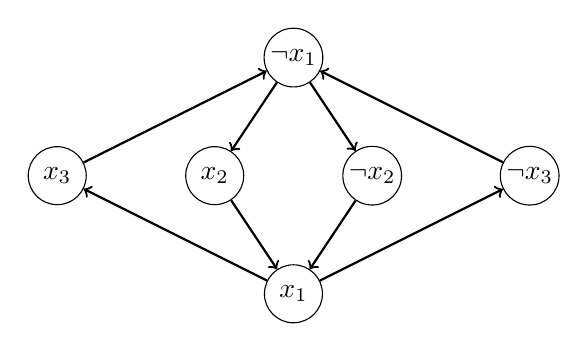
\begin{tikzpicture}[scale=1.0,minimum size=2pt]
\node[draw, circle] (1) at (1,2) {$x_3$};
\node[draw, circle] (2) at (3,2) {$x_2$};
\node[draw, circle, inner sep=1.3pt] (3) at (5,2) {$\lnot x_2$};
\node[draw, circle, inner sep=1.3pt] (4) at (7,2) {$\lnot x_3$};
\node[draw, circle, inner sep=1.3pt] (5) at (4,3.5) {$\lnot x_1$};
\node[draw, circle] (6) at (4,0.5) {$x_1$};

\path[draw,thick,->] (1) -- (5);
\path[draw,thick,->] (4) -- (5);
\path[draw,thick,->] (6) -- (1);
\path[draw,thick,->] (6) -- (4);
\path[draw,thick,->] (5) -- (2);
\path[draw,thick,->] (5) -- (3);
\path[draw,thick,->] (2) -- (6);
\path[draw,thick,->] (3) -- (6);
\end{tikzpicture}
\end{center}

ساختار گراف امکان مقداردهی درست به متغیرها را مشخص می‌کند.
شرط لازم و کافی: هیچ دو گره $x_i$ و $\lnot x_i$ داخل یک مولفه قویا همبند مشترک نباشند.
اگر باشند، مسیر بین $x_i$ به $\lnot x_i$ و برعکس هست؛ یعنی هر دو باید درست باشند، که تناقض است.

گراف $L_1$: هیچ $x_i$ و $\lnot x_i$ در یک مولفه قویا همبند نیستند؛ جواب دارد.
گراف $L_2$: همه گره‌ها در یک مولفه قویا همبند مشترک هستند؛ جواب ندارد.

یافتن مقادیر متغیرها در صورت وجود جواب: پیمایش گره‌های گراف مولفه‌ها با مرتب‌سازی توپولوژیکی معکوس.
هر مرحله: پردازش مولفه‌ای بدون یال خروجی به مولفه پردازش‌نشده.
متغیرهای مولفه اگر بیست‌مقدار باشند، طبق مولفه مقدار می‌گیرند. اگر مقدار دارند، بدون تغییر می‌مانند.
تکرار تا مقداردهی به همه متغیرها.

گراف مؤلفه‌ها برای فرمول $L_1$ بدین صورت است:
\begin{center}
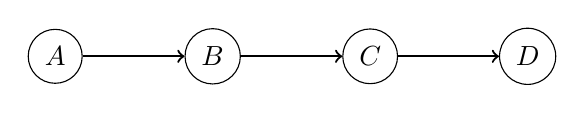
\begin{tikzpicture}[scale=1.0]
\node[draw, circle] (1) at (0,0) {$A$};
\node[draw, circle] (2) at (2,0) {$B$};
\node[draw, circle] (3) at (4,0) {$C$};
\node[draw, circle] (4) at (6,0) {$D$};

\path[draw,thick,->] (1) -- (2);
\path[draw,thick,->] (2) -- (3);
\path[draw,thick,->] (3) -- (4);
\end{tikzpicture}
\end{center}

مؤلفه‌ها عبارتند از:
$A = \{\lnot x_4\}$،
$B = \{x_1, x_2, \lnot x_3\}$،
$C = \{\lnot x_1, \lnot x_2, x_3\}$ و
$D = \{x_4\}$.
هنگام ساخت پاسخ،
ابتدا مؤلفه $D$ پردازش می‌شود
که در آن $x_4$ مقدار درست (true) می‌گیرد.
سپس مؤلفه $C$ پردازش می‌شود
که در آن $x_1$ و $x_2$ نادرست (false)
و $x_3$ درست می‌شوند.
تمام متغیرها مقداردهی شده‌اند،
بنابراین مؤلفه‌های باقی‌مانده $A$ و $B$
مقدار متغیرها را تغییر نمی‌دهند.

توجه شود این روش کار می‌کند، زیرا
گراف ساختار ویژه‌ای دارد:
اگر مسیرهایی از گره $x_i$ به گره $x_j$
و از گره $x_j$ به گره $\lnot x_j$ وجود داشته باشد،
گره $x_i$ هرگز درست نمی‌شود.
دلیل این است که مسیری نیز از گره $\lnot x_j$ به گره $\lnot x_i$ وجود دارد،
و هر دو متغیر $x_i$ و $x_j$ نادرست می‌شوند.

\index{مسئله 3SAT@مسئله 3SAT}

مسئله دشوارتر \key{مسئله 3SAT} است،
که در آن هر بخش فرمول به شکل
$(a_i \lor b_i \lor c_i)$
است.
این مسئله NP-hard است، بنابراین الگوریتم کارآمدی
برای حل آن شناخته نشده است.